%!TEX TS-program = xelatex

\documentclass[hidelinks,11pt]{friggeri-cv}
\usepackage{fontawesome}
\usepackage{tikz}
\usepackage{url}
\usepackage{color}
\usepackage{graphicx}
\usepackage{changepage}
\usetikzlibrary{decorations.markings}

\newenvironment{experience}{\begin{adjustwidth}{-4.6cm}{}}{\end{adjustwidth}}

\newfontfamily{\FA}[Path = fonts/]{FontAwesome}
\def\twitter{{\FA \faTwitter}}
\def\github{{\FA \faGithub}}
\def\linkedin{{\FA \faLinkedin}}
\def\envelope{{\FA \faEnvelope}}
\def\phone{{\FA \faPhone}}
\def\mobilePhone{{\FA \faMobilePhone}}
\def\book{{\FA \faBook}}
\def\flask{{\FA \faFlask}}
\def\search{{\FA \faSearch}}
\def\users{{\FA \faUsers}}
\def\pencil{{\FA \faPencil}}
\def\suitcase{{\FA \faSuitcase}}
\def\quotesymbol{{\FA \faQuote}}
\def\apple{{\FA \faApple}}
\def\windows{{\FA \faWindows}}
\def\linux{{\FA \faLinux}}
\def\circle{{\FA \faCircleFilled}}
\def\circleo{{\FA \faCircleO}}
\def\circlehalfo{{\FA \faCircleHalfO}}
\def\star{{\FA \faStar}}
\def\staro{{\FA \faStarEmpty}}
\def\starhalfo{{\FA \faStarHalfO}}
\def\user{{\FA \faUser}}

\newcommand{\printaside}{
  \begin{aside}
  	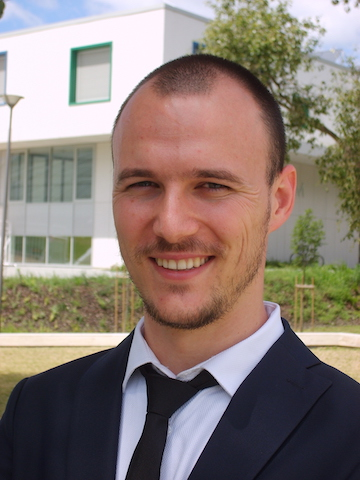
\includegraphics[width=3.3cm,keepaspectratio]{images/photo.jpg}
    \section{Favourite tool set}\\
    {
      Java 8 - 15 {\footnotesize \textcolor{gray}{\star\star\staro}}\\
      Spring {\footnotesize \textcolor{gray}{\star\star\staro}}\\
      Kotlin (wishlist) {\footnotesize \textcolor{gray}{\star\star\staro}}\\
      PostgreSQL {\footnotesize \textcolor{gray}{\star\star\staro}}\\
      Intellij Idea {\footnotesize \textcolor{gray}{\star\star\staro}}\\
      Bash {\footnotesize \textcolor{gray}{\star\starhalfo\staro}}\\
      Docker {\footnotesize \textcolor{gray}{\star\star\star}}\\
      Git {\footnotesize \textcolor{gray}{\star\star\star}}\\
      Github {\footnotesize \textcolor{gray}{\star\star\staro}}\\
     }
    \section{Operating systems}\\
      Linux \textcolor{gray}{\linux}\\\
      Mac OS X \textcolor{gray}{\apple}\\\
      Windows \textcolor{gray}{\windows}\\
    \section{Languages}\\
    {
      English
\includegraphics[width=0.4cm,keepaspectratio]{images/uk.png}\\
    	Hungarian
\includegraphics[width=0.4cm,keepaspectratio]{images/hu.png}\\
    	Romanian
\includegraphics[width=0.4cm,keepaspectratio]{images/ro.png}\\
    }
    \section{Contact}{
    	~\\
    	\textcolor{gray}{\mobilePhone} +41 76 233 2746\\\
    	\href{mailto:laslaul@yahoo.com}{\textcolor{gray}{\envelope} laslaul@yahoo.com}\\
    	\href{https://github.com/LeonardLaszlo}{\textcolor{gray}{\github} LeonardLaszlo}\\
    	\href{http://www.linkedin.com/in/LeonardLaszlo}{\textcolor{gray}{\linkedin} Leonard László}\\
    	~\\
    	\href{https://goo.gl/maps/hmDQ8qNK5KMDU4kh9}{
    		{\Large Leonard László}\\
    		8134 Adliswil,\\
        Switzerland\\
    	}
    }
  \end{aside}
}

\begin{document}
\header{\thinfont Leonard\ }{\boldfont László}{Senior Computer Engineer}
\printaside

\section{{\user} Recommendation \hfill {\small Péter Módos, Tech lead @ SimpledCard,
\href{http://www.linkedin.com/in/LeonardLaszlo}{LinkedIn}, July 4th, 2019)}}
\textit{„Leonard worked in my team at SimpledCard as a Java developer. He is very passionate about technology,
he doesn't stop programming at the end of the working day, he keeps playing with new technologies also at home.
As a result, he is quite up-to-date about new solutions and trends and he is happy to apply his ideas at work.
He is constantly challenging the status quo, he is the driver of a lot of improvements.
He likes to understand the business aspects of the work as well, which would make him a productive and dedicated
contributor of any software projects.“}

\section{{\suitcase}\ Experience Summary}
\begin{entrylist}
    \entry
    {2019--}
    {Software Engineer}
    {Move Digital AG, Zurich}
    {Currently working on the development of a quoting system for financial products.}
    \entry
    {2017--2019}
    {Software Engineer}
    {SimpledCard, Budapest}
    {Worked on SimpledCard product, a Dutch enterprise electronic payment system.}
    \entry
    {2016--2017}
    {Software Engineer}
    {Evosoft, Budapest}
    {Worked on Mindsphere product, a Big Data IoT cloud platform for Siemens.}
    \entry
    {2014}
    {Software Engineer}
    {Siwena, Budapest}
    {Developed a Java library for communication with SNMP compatible devices.}
    \entry
    {2013}
    {Safety-Critical System Tester}
    {Testware, Budapest}
    {Tested the safety-critical operating system of Alstom's self-driving trains, metros and trams.}
    \entry
    {Always}
    {SBC enthusiast}
    {}
    {Author of \textit{\href{https://github.com/LeonardLaszlo/nw.js-armv7-binaries}{NW.js for ARMv7}} and other
    \textit{\href{http://www.hardkernel.com/main/main.php}{Odroid}} and \textit{\href{https://www.raspberrypi.org}{Rpi}}
    single-board computer projects, such as the collection and visualisation of data points, git backbone repositories
    setups, database setups, file server setups and web server setups.}
\end{entrylist}

\section{{\pencil}\ Education}
\begin{entrylist}
  \entry
    {2015--2016}
    {{\normalfont Computer engineering M.Sc.}}
    {\href{http://www.bme.hu/?language=en}{Budapest University of Technology and Economics}
    (\href{https://www.aut.bme.hu/en/default.aspx}{BME--AUT})}
    {Thesis title: Multi-platform multimedia application development with
    \textit{\href{https://nwjs.io/}{NW.js}} framework.}
  \entry
    {2011--2015}
    {{\normalfont Computer engineering B.Sc.}}
    {\href{http://www.bme.hu/?language=en}{Budapest University of Technology and Economics}
    (\href{http://www.mit.bme.hu/eng/}{BME--MIT})}
    {Specialized in system design. Thesis title: Cloud monitoring solutions.}
\end{entrylist}

\section{{\book}\ Publications}
Multi-platform multimedia application development with NW.js framework.

Porting Popcorn Time for ARMv7 Linux devices.
{\small (Odroid Magazine, July 2015, \textit{\href{http://bit.ly/29G47yN}{http://bit.ly/29G47yN}})}

Proxying Popcorn Time API calls.

\newpage

\header{\thinfont Leonard\ }{\boldfont László}{Senior Computer Engineer}
\begin{experience}

{\LARGE Software Engineer at Move Digital, Zurich (Sep. 2019 - Ongoing)}

Currently I work on the development of a quoting system for financial products, where I use on a daily basis the following technologies:

\begin{itemize}
	\item Java 11, Spring Boot 2.2.x, Docker, Bash, Git, Github, Maven, Jenkins, Jira, Confluence, Intellij Idea
	\item MariaDB, PostgreSQL, ArangoDB, RabbitMQ, MinIO, Redis
  \item Elasticsearch, Logstash, Kibana, Beats, Websockets
\end{itemize}

My most significant contributions are in the implementation of financial products and trading workflows in Java.
Other personal accomplishments are: improving the coding guidelines, enabling most of the current Checkstyle and PMD rules, introduction of the ELK stack for monitoring and influencing the architectural and technological decisions.

{\LARGE Software Engineer at SimpledCard, Budapest (Oct. 2017 - Feb. 2019)}

At SimpledCard I worked in a small and highly efficient team with continuously improving processes.
I learned to accept and offer honest feedback and the importance of building tech culture in the team.
My role included the development of the payment system, fixing all the errors from the logs, feature design and specification, executing weekly releases and monitoring.
Other personal accomplishments include the migration from Java 7 to Java 8 and the automation of some manual back-office processes. The tech stack included:

\begin{itemize}
	\item Java 7 and 8, Spring Boot 1.5.x, AWS (SNS, SES, SQS S3, EC2, RDS, Cloud formation), PostgreSQL
	\item Vert.x (v2.x), Guice, Junit, Hamcrest, Bash, Maven, Git, Circle CI, Intellij Idea
\end{itemize}

{\LARGE Software Engineer at Evosoft, Budapest (Sep. 2016 - Oct. 2017)}

At Evosoft I worked on the Mindsphere project, which taught me many valuable lessons that influenced my career and helped me build many long lasting friendships.
I mostly worked on the development of the API gateway, and when needed I partly took over the leading of my team which resulted in a promotion to a senior position.
I frequently worked with:

\begin{itemize}
	\item Java 8, Spring Boot 1.5.x, PostgreSQL, MongoDB, RabbitMQ, Redis, Node.js, Cloud Foundry, Gradle, Git, Gitlab CI
	\item Intellij Idea, TestNG, test-driven development, pair programming and custom agile processes.
\end{itemize}

{\LARGE Software Engineer at Siwena, Budapest (2014)}

Siwena is a monitoring system with notable clients, such as the Liszt Ferenc International Airport and the nuclear power plant at Paks.
It is used to process data from cameras, motion detectors, locks and sensors.
My contribution to the project was the design and implementation of a library for the communication with SNMP compatible devices.
We used the classic Java SE stack.

{\LARGE Testing Engineer at Testware, Budapest (2013)}

At Testware I tested Ada and C code running on Alstom's self-driving trains, metros and trams with IBM's RTRT.

{\LARGE About me}

I am a backend Software Engineer with 5+ years of experience with Java and its ecosystem.
When it suits the task better or when I have the freedom to try something new I also use other programming languages and tools.
For me the foundation of a good company culture means honest and clear communication, trust, constructive passionate debate, commitment, accountability and attention to results.
I like to pay attention to clean code, cover my work with tests, being involved in the planning process, architecture decisions, specifications and reviewing the code of my peers.
One of my most popular open-source projects is \href{https://github.com/LeonardLaszlo/nw.js-armv7-binaries}{\textit{NW.js for ARMv7}}.

SSBoYW5kbGUgZW1haWxzIGF0IGxlb25hcmQubGFzemxvQGdtYWlsLmNvbSB3aXRoIGhpZ2ggcHJpb3JpdHku

\end{experience}

\end{document}
